\chapter{Discussion}
Please tell more about conclusion and how to the next work of this study.

\section{Rahmi Roza-1164085}
\subsection{Teori}
\begin{enumerate}
\item Kenapa File Suara Harus Dilakukan MFCC
\begin{itemize}
\item Penjelasan: Agar bisa mengubah suara menjadi vektor. Sehingga data suara bisa diolah menjadi outputan. Jadi semua parameter inputan baik itu suara, dokumen harus dipersiapkan datanya terlebih dahulu, kalau untuk dokumen untuk teks menggunakan word2vec, sedangkan untuk suara menggunakan MFCC (Mel Frequency Cepstral Coeficients) 
\par 
\par
\item Ilustrasi Gambar
\begin{figure}[!hbtp]
\centering
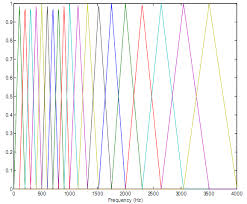
\includegraphics[scale=0.7]{figures/mfccroza.jpg}
\caption{MFCC Roza}
\label{text-fadila}
\end{figure}
\par
\end{itemize}
\par
\par

\item Konsep Dasar Neural Network
\begin{itemize}
\item  Penjelasan:
\par Neural Network merupakan kategori ilmu Soft Computing. Neural Network sebenarnya mengadopsi dari kemampuan otak manusia yang mampu memberikan stimulasi/rangsangan, melakukan proses, dan memberikan output. Output diperoleh dari variasi stimulasi dan proses yang terjadi di dalam otak manusia. Kemampuan manusia dalam memproses informasi merupakan hasil kompleksitas proses di dalam otak. Misalnya, yang terjadi pada anak-anak, mereka mampu belajar untuk melakukan pengenalan meskipun mereka tidak mengetahui algoritma apa yang digunakan.
\par
\item Ilustrasi Gambar
\begin{figure}[!hbtp]
\centering
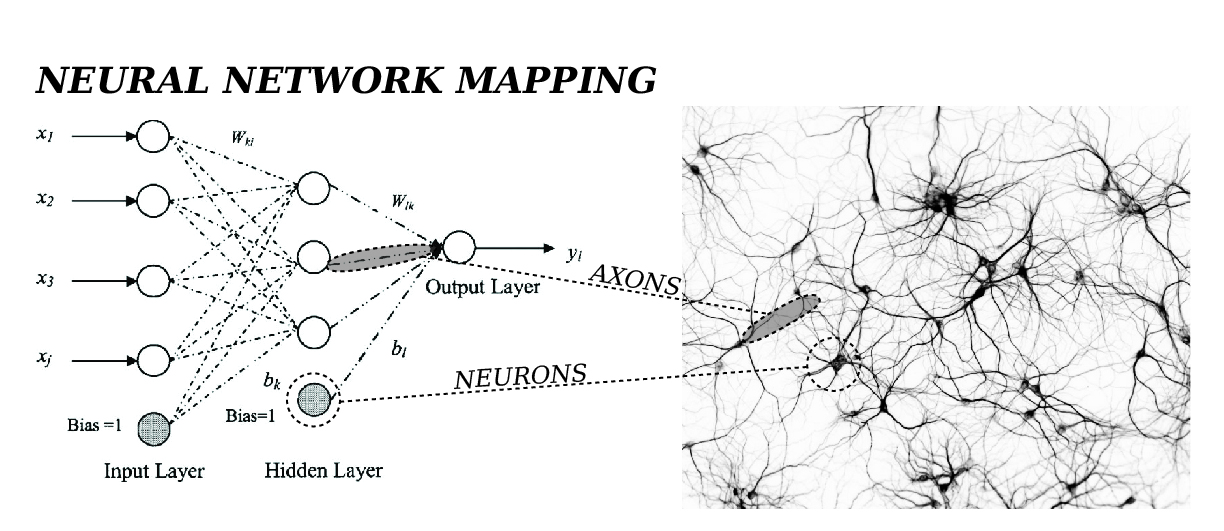
\includegraphics[scale=0.3]{figures/neuralroza.jpg}
\caption{Konsep Dasar Neural Network Roza}
\label{text-fadila}
\end{figure}
\par
\end{itemize}
\par
\par

\item Konsep Pembobotan Dalam Neural Network
\begin{itemize}
\item Penjelasan:
\par Cara kerja Neural Network dapat dianalogikan sebagaimana halnya manusia belajar dengan mengunakan contoh atau yang disebut sebagai supervised learning. Sebuah Neural Network dikonfigurasi untuk aplikasi tertentu, seperti pengenalan pola atau klasifikasi data, dan kemudian disempurnakan melalui proses pembelajaran. Proses belajar yang terjadi dalam sistem biologis melibatkan penyesuaian koneksi sinaptik yang ada antara neuron, dalam halnya pada Neural Network penyesuaian koneksi sinaptik antar neuron dilakukan dengan menyesuaikan nilai bobot yang ada pada tiap konektivitas baik dari input, neuron maupun output.
\par
\item Ilustrasi Gambar
\begin{figure}[!hbtp]
\centering
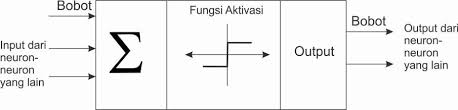
\includegraphics[scale=0.5]{figures/pemboobotanroza.jpg}
\caption{Konsep Pembobotan Roza}
\label{text-fadila}
\end{figure}
\par
\end{itemize}
\par
\par

\item Konsep Fungsi Aktivasi Dalam Neural Network
\begin{itemize}
\item Penjelasan:
\par Setiap neuron mempunyai tingkat aktivasi yang merupakan fungsi dari input yang masuk padanya. Aktivasi yang dikirim suatu neuron ke neuron lain berupa sinyal dan hanya dapat mengirim sekali dalam satu waktu, meskipun sinyal tersebut disebarkan pada beberapa neuron yang lain.
\par
\item Ilustrasi Gambar
\begin{figure}[!hbtp]
\centering
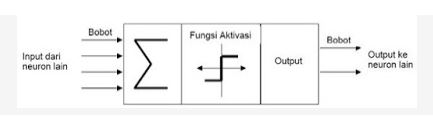
\includegraphics[scale=0.7]{figures/aktivasiroza.jpg}
\caption{Konsep Aktivasi Roza}
\label{text-fadila}
\end{figure}
\par
\end{itemize}
\par
\par

\item Cara Membaca Hasil Plot Dari MFCC
\begin{itemize}
\item Penjelasan:
\par Nanti akan ada outputan berbentuk grafik. Ada 3 dimensi atau sumbu. Dimana untuk sumbu x merupakan waktu, sedangkan sumbu y merupakan frekuensi dari suara yang dihasilkan dalam bentu Hz. Sedangkan pada bagian tengah atau sumbu z merupakan power atau kekuatan dari lagu atau suara atau desibel yang dihasilkan. Untuk melihat penjelasan dari warna pada gambar yang di tengah, maka kita harus mendownload gambar nya terlebih dahuhulu. Untuk warna biru itu merupakan suara rendah, yang merah merupakan tinggi dan daya frekuensi nya berada pada nilai yang rendah karena bass bekerja pada suara yang rendah. Tidak selalu tergantung pada warna untuk menentukan nilai atau frekuensinya. Tetapi pada jenis lagu yang dugunakan. 
\par
\item Ilustrasi Gambar
\begin{figure}[!hbtp]
\centering
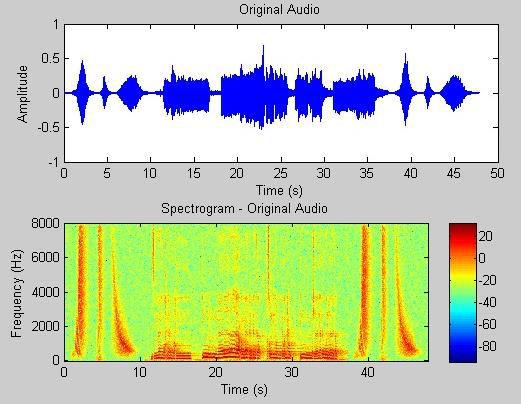
\includegraphics[scale=0.5]{figures/caramembacaroza.jpg}
\caption{Cara Membaca Hasil Plot MLCC Roza}
\label{text-fadila}
\end{figure}
\par
\end{itemize}
\par
\par



\item Apa Itu One-Hot Encoding?
\begin{itemize}
\item Penjelasan:
\par One-hot encoding adalah representasi dari variabel kategori sebagai vektor biner. Yang pertama adalah  mengharuskan nilai kategorikal dipetakan ke nilai integer. Kemudian, setiap nilai integer direpresentasikan sebagai vektor biner yang semuanya bernilai nol kecuali indeks integer, yang ditandai dengan 1.
\par
\item Ilustrasi Gambar
\begin{figure}[!hbtp]
\centering
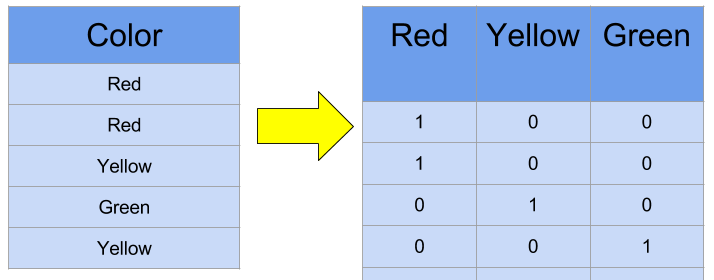
\includegraphics[scale=0.5]{figures/onehotroza.png}
\caption{One Hot Encoding Roza}
\label{bag-fadila}
\end{figure}
\par
\end{itemize}
\par
\par

\item Fungsi Dari np unique dan to categorical dalam kode program
\begin{itemize}
\item  Np.unique
\par 
\item Penjelasan: Untuk mengekstaksi elemen-elemen unik (tertentu) dalam array.
\begin{figure}[!hbtp]
\centering
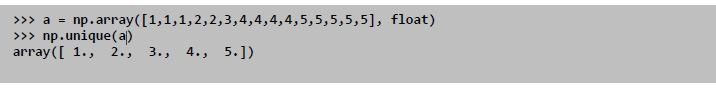
\includegraphics[scale=0.7]{figures/npuniqueroza.jpg}
\caption{NP Unique Roza}
\label{tf-fadila}
\end{figure}
\par
\end{itemize}
\par
\begin{itemize}
\item  To categorical
\par 
\item Penjelasan: Berfungsi untuk mengubah vektor kelas yang berupa integer ( number ) menjadi matriks kelas biner.	
\begin{figure}[!hbtp]
\centering
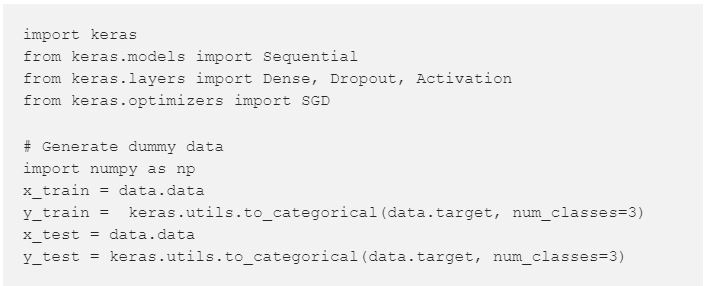
\includegraphics[scale=0.7]{figures/tocategorical.jpg}
\caption{To Categorical roza}
\label{tf-fadila}
\end{figure}
\par
\end{itemize}
\par
\par

\item Fungsi Dari Sequential Pada Kode Program
\begin{itemize}
\item Penjelasan:
\par Sequential proses membandingkan setiap elemen larik satu per satu secara beruntun, mulai dari elemen pertama, sampai dengan elemen terakhir atau elemen yang dicari sudah ditemukan. atau merupakan jenis model yang digunakan dalam perhitungan ataupun code program yang direalisasikan.
\par
\item Ilustrasi Gambar
\begin{figure}[!hbtp]
\centering
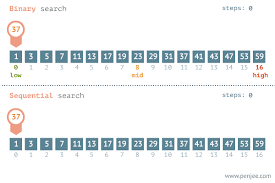
\includegraphics[scale=0.8]{figures/sequentialroza.png}
\caption{Sequential Roza Roza}
\label{text-fadila}
\end{figure}
\par
\end{itemize}
\par
\par

\begin{itemize}
\item Plagiarisme Roza
\begin{figure}[!hbtp]
\centering
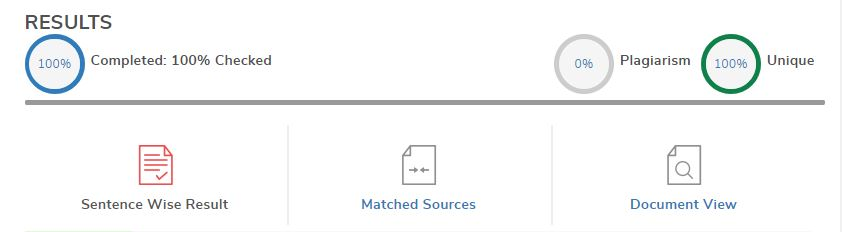
\includegraphics[scale=0.5]{figures/plagiarisme.jpg}
\caption{Plagiarisme Roza}
\label{text-fadila}
\end{figure}
\end{itemize}

\end{enumerate}